\subsection{Context}
The database exists to store the images used by the neural network, including training data, and data collected at runtime for future training and testing. Images will generally be added one at a time during runtime, but during testing and development the capability to add several, potentially hundreds of images per transaction. 

\subsection{Dependancies} 
The database will not depend on any other subsystem for opperation.

\subsection{Structure}
Making use of SQLite, the database itself will consist of a single file, alongside a folder containing the named image files. The database will consist of a single table consisting of the following columns: index (integer), image address (String), actual type(boolean), guessed type (boolean). While not in use, this foder could be compressed into a tar archive.


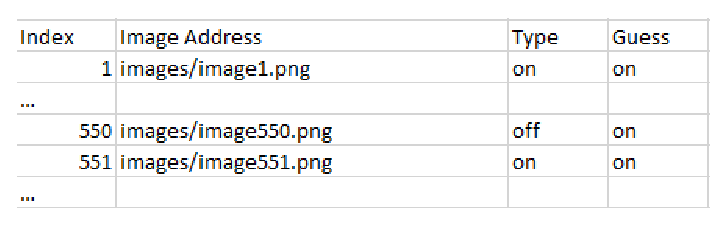
\includegraphics[height=4cm]{dbexample}

\subsection{Logical}

The database will be coded to support the following functions:

\begin{minted}{Java}

public class Fibonacci {
 
  // The golden ratio $\phi = \frac{1 + \sqrt{5}}{2}$.
  public static final double PHI = (1.0 + Math.sqrt(5.0)) / 2.0;
 
  public static double fibonacci(long n) {
    if (n \&lt; 0) throw new IllegalArgumentException();
    return Math.floor(Math.pow(PHI, n) / Math.sqrt(5.0) + 0.5);
  }
 
}


\end{minted}


